The El Gamal cryptosystem is a public key cryptosystem based on the
difficulty of computing discrete logarithms in cyclic groups.

The cryptosystem is defined over a group $G_q$ of order $q$ with
generator $g$. The secret key $x$ is chosen randomly in $\mathbb{Z}_q$
and the public key $y$ is created as follows
$$
y = g^x
$$

Encryption of a plaintext $m \in G_q$ is done by choosing a random $s
\in \mathbb{Z}_q$ and computing
$$
\mathrm{Enc}(m,s) = (u,v) = (g^s, y^sm) \in G_q \times G_q
$$

Decryption of a ciphertext $(u,v) \in G_q \times G_q$ is achieved by
using the private key $x$ to compute
$$ 
\mathrm{Dec}(u,v) = u^{-x}v = (g^s)^{-x}y^sm = (g^x)^{-s}y^sm = y^{-s}y^sm = m
$$

The El Gamal cryptosystem possesses a homomorphic property. This means
that for two messages $m_1,m_2 \in G_q$ and random numbers $s_1, s_2
\in \mathbb{Z}_q$
$$
\mathrm{Enc}(m_1,s_1) \cdot \mathrm{Enc}(m_2,s_2) = \mathrm{Enc}(m_1m_2,s_1 + s_2)
$$

By choosing one of the messages to be the identity element, $m_2 = 1$,
and letting the other one being any message $m_1 = m$, one has
obtained the ability to reencrypt a particular ciphertext without
knowing the original plaintext nor the randomness. 
$$
\mathrm{Enc}(m,s_1) \cdot \mathrm{Enc}(1,s_2) = \mathrm{Enc}(m_1, s_1 + s_2)
$$

This property of a cryptosystem is necessary if it should be used in a
reencryption mix-net.


\begin{center}
  \makebox[\textwidth]{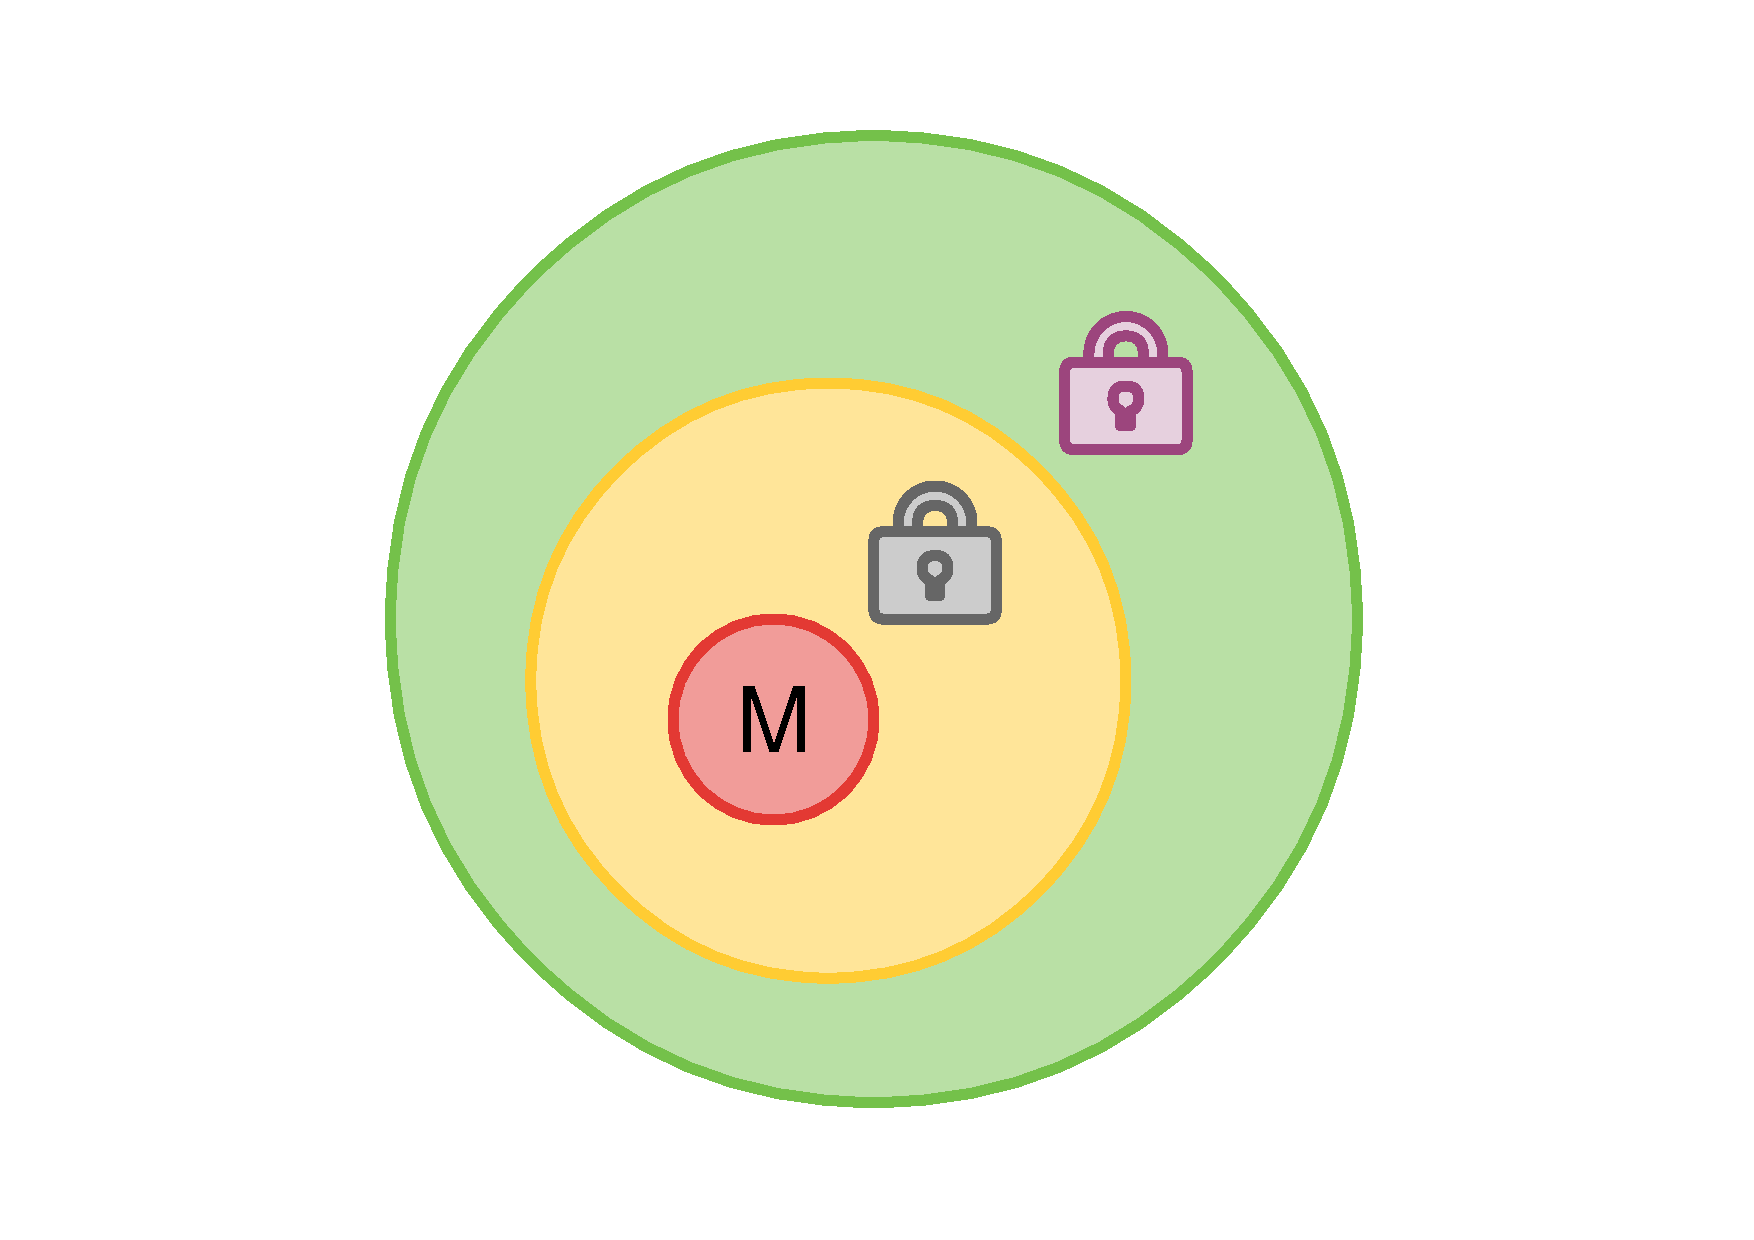
\includegraphics[width=0.3\textwidth]{../presentation/images/mix6.pdf}}
\end{center}
